\documentclass{article}
\usepackage[a4paper, left=3cm, right=2cm, top=2cm, bottom=2cm]{geometry}
\usepackage[brazil]{babel}
%\usepackage[utf8]{inputenc} % Por alguma raz�o diab�lica estava dando problema com os encodes
\usepackage[T1]{fontenc}

\usepackage{parskip} % Para remover identa��o desnecessaria.

\usepackage{amsmath} % Para poder usar \implies

\usepackage{pdfpages}

\usepackage{lipsum}

\newcommand{\myspace}{0.5cm}

\begin{document}
\pagenumbering{gobble}

1. Dados: $\mathrm{Q =  \ m^{3}/s}$, $\mathrm{T =  ^{\circ}C}$, $\mathrm{g =  \ m/s^{2}}$. Escolhendo a calha parshal com as seguintes dimens�es: $\mathrm{W =  \ m}$, $\mathrm{C =  \ m}$,  $\mathrm{D =  \ m}$, $\mathrm{N =  \ m}$, $\mathrm{k =  }$, $\mathrm{n =  \ m}$ \\

2. Calculo da velocidade e da profundidade da �gua na se��o de medi��o (se��o 0):

\vspace{\myspace}

\begin{center}
	$
		\mathrm
		{
			H_{0} = kQ^{n}
		}
		\implies
		\mathrm
		{
			H_{0} =  \cdot ^{  }
		} 
		\implies 
		\fbox
		{ 
			$\mathrm
			{
				H_{0} =  \ m
			}$
		} 
	$
\end{center}

\vspace{\myspace}

\begin{center}
	$
		\mathrm
		{
			D_{0} = \dfrac{2}{3} \left ( D - W \right ) + W
		} 
		\implies
		\mathrm
		{
			D_{0} = \dfrac{2}{3} \left (  -  \right ) + 
		}
		\implies 
		\fbox
		{ 
			$\mathrm
			{	
				D_{0} =  \ m
			}$
		} 
	$	
\end{center}

\vspace{\myspace}

\begin{center}
	$
		\mathrm
		{
			U_{0} = \dfrac{Q}{D_{0}H_{0}}
		} 		
		\implies 
		\mathrm
		{
			U_{0} = \dfrac{  }{  \cdot  }
		}
		\implies 
		\fbox
		{ 
			$\mathrm
			{
				U_{0} =  \ m/s
			}$
		}
	$  	
\end{center}

\vspace{\myspace}

3. Vaz�o especifica na garganta da Calha Parshall:

\vspace{\myspace}

\begin{center}
	$ 
		\mathrm
		{
			q = \dfrac{Q}{W}
		}
		\implies 
		\mathrm
		{
			q = \dfrac{  }{  }			
		}
		\implies 
		\fbox
		{
		 	$\mathrm
		 	{	
		 		q =  \ m^{3}\cdot s^{-1}/m
		 	}$
		 }
	$
\end{center}

\vspace{\myspace}

4. Carga hidr�ulica dispon�vel:

\vspace{\myspace}

\begin{center}
	$
		\mathrm
		{
			E_{0} = \dfrac{U_{0}^{2}}{2g} + H_{0} + N 
		} 
		\implies 
		\mathrm
		{
			E_{0} = \dfrac{ ^{2}}{2\cdot  } +  +  
		}
		\implies
		\fbox
		{ 
			$\mathrm
			{
				E_{0} =  \ m
			}
			$
		} 
	$  
\end{center}

\vspace{\myspace}

5. Carga hidr�ulica dispon�vel.\\

\vspace{\myspace}

Seja: $ \mathrm{x = -gq\left ( \dfrac{2}{3} gE_{0}\right )^{-1.5}}$. Manipulando a express�o, tem-se:

\vspace{\myspace}

\begin{center}
	$	
		\mathrm
		{
			\cos \! \left ( \theta \right ) =x 
			\implies  
			\theta=\arccos \! \left ( x \right ) 
			\implies 
			\dfrac{\theta}{3}=\ \dfrac{\arccos\left ( x \right )}{3} 
			\implies 
			\cos \! \left ( \dfrac{\theta}{3} \right ) = \cos \! \left ( \dfrac{\arccos \! \left( x \right )}{3} \right)
		}
	$
\end{center}

\vspace{\myspace}

Montando uma s� express�o para a determinar a velocidade $\mathrm{U_{1}}$: 

\vspace{\myspace}

\begin{center}
	$	
		\mathrm
		{
			U_{1}=2\sqrt{\dfrac{2gE_{0}}{3}}\cos \! \left (\dfrac{1}{3}\arccos \! \left( -gq\left [\left ( \dfrac{2}{3} gE_{0}\right )^{-1.5}  \right ] \right ) \right)
		}
	$
\end{center}

\vspace{\myspace}

Substituindo-se os valores:

\vspace{\myspace}

\begin{center}
	$
		\mathrm
		{
			U_{1}=2\sqrt{\dfrac{2 \cdot  \cdot  }{3}}\cos \! \left (\dfrac{1}{3}\arccos \! \left( -  \cdot  \left [\left ( \dfrac{2}{3}\cdot  \cdot  \right )^{-1.5}  \right] \right ) \right)
		}
	$
\end{center}

\vspace{\myspace}

\begin{center}
	$
		\fbox
		{
			$
				\mathrm{U_{1}}=  \mathrm{\ m/s}
			$
		}
	$
\end{center}

\vspace{\myspace}

Calculando $ \mathrm{h_{1}}$:

\vspace{\myspace}

\begin{center}
	$
		\mathrm
		{
			h_{1}= \dfrac{q}{U_{1}}
		} 
		\implies
		\mathrm
		{
			h_{1}= \dfrac{  }{  }
		}
		\implies
		\fbox{ 
			$
				\mathrm
				{
					h_{1}=  \ m
				}
			$  
		}
	$
\end{center}

\vspace{\myspace}

6. N�mero de Froud:	

\vspace{\myspace}

\begin{center}
	$
		\mathrm
		{
			F_{1} = \dfrac{U_{1}}{\sqrt{gh}}
		}
		\implies
		\mathrm
		{
			F_{1} = \dfrac{  }{\sqrt{  \cdot  }}
		}
		\implies 
		\fbox
		{
			$\mathrm
			{
				F_{1} =  
			}$
		}
	$  
\end{center}

\vspace{\myspace}

7. C�lculo da altura do conjugada do ressalto (se��o 2):

\vspace{\myspace}

\begin{center}
	$
		\mathrm
		{
			h_{2} = \dfrac{h_{1}}{2}\left ( \sqrt{1+ 8F_{1}^{2}} - 1\right )
		}
		\implies 
		\mathrm
		{
			h_{2} = \dfrac{  }{2}\left ( \sqrt{1+ 8\cdot  ^{2}} - 1\right )
		}
		\implies 
		\fbox
		{
			$\mathrm
			{
				h_{2} =  \ m
			}$
		}
	$
\end{center}

\vspace{\myspace}

8. Profundidade e da velocidade d'�gua na se��o de sa�da (se��o 3):

\vspace{\myspace}

\begin{center}
	$
		\mathrm
		{
			h_{3} = h_{2} - \left ( N - K \right )
		} 
		\implies
		\mathrm
		{
			h_{3} =  - \left (  -  \right )
		}
		\implies 
		\fbox
		{
			$\mathrm
			{	
				h_{3} =  \ m
			}$
		}
	$  
\end{center}

\vspace{\myspace}

\begin{center}
	$
		\mathrm
		{
			U_{3} = \dfrac{Q}{Ch_{3}}
		} 
		\implies
		\mathrm
		{
			U_{3} = \dfrac{  }{  \cdot  }
		}
		\implies 
		\fbox
		{	
			$\mathrm
			{
				U_{3} =  \ m
			}$
		}
	$ 
\end{center}

\vspace{\myspace}

9. Extens�o do ressalto e perda de carga: *Falta modificar 
% L = 4\left ( h_{2} - h_{1} \right) , se F1 for pequeno<4.5
% L = 6\left ( h_{2} - h_{1} \right) , se F1 for 4,5 < F1 < 16

\vspace{\myspace}

\begin{center}
	$
		\mathrm
		{
			L = 6\left ( h_{2} - h_{1} \right)
		} 
		\implies
		\mathrm
		{
			L = 6\left (  -  \right)
		}
		\implies 
		\fbox
		{ 
			$\mathrm
			{
				L =  \ m
			}$
		}
	$
\end{center}

\vspace{\myspace}

\begin{center}
	$
		\mathrm
		{
			h = \dfrac{\left ( h_{2} - h_{1} \right)^{3}}{4h_{1}h_{2}} 
		} 
		\implies
		\mathrm
		{
			h = \dfrac{\left (  -  \right)^{3} }{4\cdot  \cdot  } 
		}
		\implies 
		\fbox
		{
			$\mathrm
			{
				h =  \ m
			}$
		}
	$
\end{center}

\vspace{\myspace}

10. Tempo de mistura e gradiente de velocidade:

\vspace{\myspace}

\begin{center}
	$
		\mathrm
		{
			T_{m} = \dfrac{2L}{\left ( U_{1} + U_{3} \right)}
		} 
		\implies
		\mathrm
		{
			T_{m} = \dfrac{2\cdot  }{\left (  +  \right)}
		}
		\implies 
		\fbox
		{ 
			$\mathrm
			{
				T_{m}=  \ s
			}$
		}
	$
\end{center}

\vspace{\myspace}

\begin{center}
	$
		\mathrm
		{
			G_{m} = \sqrt{\dfrac{\rho g h}{\mu T_{m}}}
		} 
		\implies
		\mathrm
		{
			G_{m} = \sqrt{\dfrac{  \cdot  \cdot   }{  \cdot  }} } 
		\implies 
		\fbox
		{
			$\mathrm
			{
				G_{m} =  \ s^{-1}
			}$
		}
	$
\end{center}

\newpage

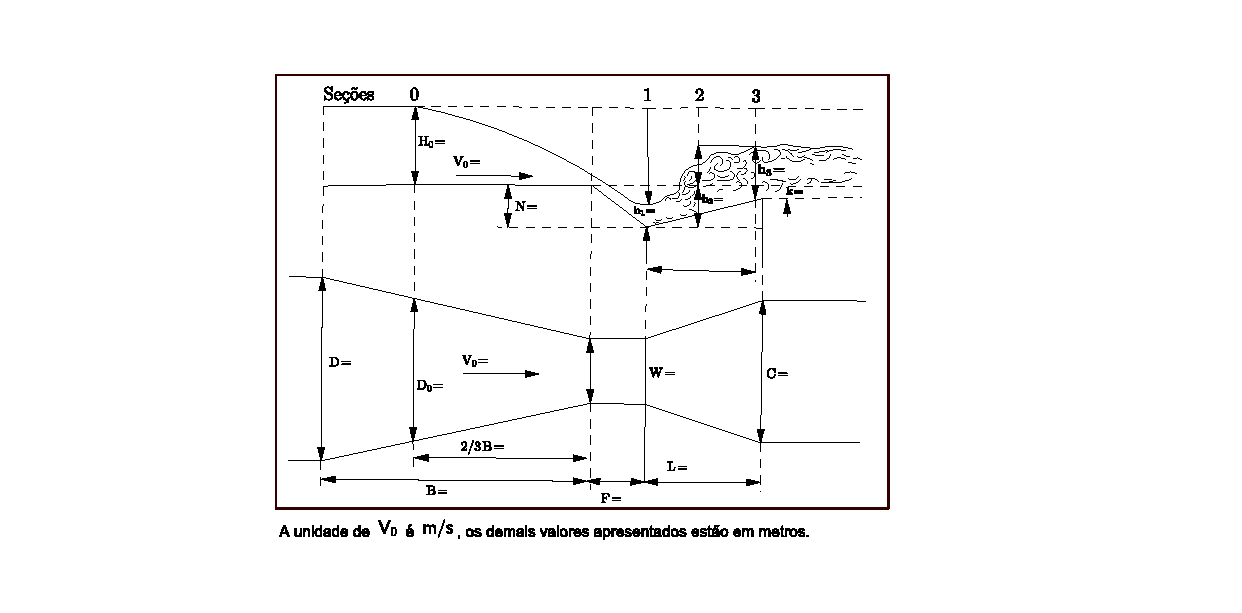
\includepdf[scale=1.8, angle=90, offset=-5mm 20mm]{calha_parshall.pdf}	


\end{document} 